% -*- Mode:TeX -*-

%% IMPORTANT: The official thesis specifications are available at:
%%            http://libraries.mit.edu/archives/thesis-specs/
%%
%%            Please verify your thesis' formatting and copyright
%%            assignment before submission. If you notice any
%%            discrepancies between these templates and the 
%%            MIT Libraries' specs, please let us know
%%            by e-mailing thesis@mit.edu

%% The documentclass options along with the pagestyle can be used to generate
%% a technical report, a draft copy, or a regular thesis. You may need to
%% re-specify the pagestyle after you \include cover.tex. For more
%% information, see the first few lines of mitthesis.cls. 

%\documentclass[12pt,vi,twoside]{mitthesis}
%%
%%  If you want your thesis copyright to you instead of MIT, use the
%%  ``vi'' option, as above.
%%
%\documentclass[12pt,twoside,leftblank]{mitthesis}
%%
%% If you want blank pages before new chapters to be labelled ``This
%% Page Intentionally Left Blank'', use the ``leftblank'' option, as
%% above. 

\documentclass[12pt,twoside,upcase]{mitthesis}
\usepackage{lgrind}
%% These have been added at the request of the MIT Libraries, because
%% some PDF conversions mess up the ligatures.  -LB, 1/22/2014
\usepackage{cmap}
\usepackage[T1]{fontenc}
\usepackage{caption}
\usepackage{subcaption}
\usepackage{graphicx}
\usepackage{hyperref}
\usepackage{color}
\pagestyle{plain}

%% This bit allows you to either specify only the files which you wish to
%% process, or `all' to process all files which you \include.
%% Krishna Sethuraman (1990).

%\typein [\files]{Enter file names to process, (chap1,chap2 ...), or `all' to process all files:}
\def\all{all}
\ifx\files\all \typeout{Including all files.} \else %\typeout{Including only \files.} \includeonly{\files} \fi
\newcommand{\code}[1]{\texttt{#1}}
\newcommand{\opera}{\cite{mellette_expanding_2019}}
\newcommand{\rotornet}{\cite{mellette_rotornet_2017}}
\newcommand{\para}[1]{\vspace{0.05in}{\bf {#1}} }
\newcommand{\manya}[1]{\textit{\textcolor{red}{Manya: #1}}}
\newcommand{\olivia}[1]{\textit{\textcolor{magenta}{Olivia: #1}}}


\graphicspath{ {./figures/} }

\begin{document}

% -*-latex-*-
% 
% For questions, comments, concerns or complaints:
% thesis@mit.edu
% 
%
% $Log: cover.tex,v $
% Revision 1.9  2019/08/06 14:18:15  cmalin
% Replaced sample content with non-specific text.
%
% Revision 1.8  2008/05/13 15:02:15  jdreed
% Degree month is June, not May.  Added note about prevdegrees.
% Arthur Smith's title updated
%
% Revision 1.7  2001/02/08 18:53:16  boojum
% changed some \newpages to \cleardoublepages
%
% Revision 1.6  1999/10/21 14:49:31  boojum
% changed comment referring to documentstyle
%
% Revision 1.5  1999/10/21 14:39:04  boojum
% *** empty log message ***
%
% Revision 1.4  1997/04/18  17:54:10  othomas
% added page numbers on abstract and cover, and made 1 abstract
% page the default rather than 2.  (anne hunter tells me this
% is the new institute standard.)
%
% Revision 1.4  1997/04/18  17:54:10  othomas
% added page numbers on abstract and cover, and made 1 abstract
% page the default rather than 2.  (anne hunter tells me this
% is the new institute standard.)
%
% Revision 1.3  93/05/17  17:06:29  starflt
% Added acknowledgements section (suggested by tompalka)
% 
% Revision 1.2  92/04/22  13:13:13  epeisach
% Fixes for 1991 course 6 requirements
% Phrase "and to grant others the right to do so" has been added to 
% permission clause
% Second copy of abstract is not counted as separate pages so numbering works
% out
% 
% Revision 1.1  92/04/22  13:08:20  epeisach

% NOTE:
% These templates make an effort to conform to the MIT Thesis specifications,
% however the specifications can change. We recommend that you verify the
% layout of your title page with your thesis advisor and/or the MIT 
% Libraries before printing your final copy.
\title{Fast packet-level datacenter network simulation}

\author{Olivia Brode-Roger}
% If you wish to list your previous degrees on the cover page, use the 
% previous degrees command:
\prevdegrees{B.S., Massachusetts Institute of Technology (2018)}
% You can use the \\ command to list multiple previous degrees
%       \prevdegrees{B.S., University of California (1978) \\
%                    S.M., Massachusetts Institute of Technology (1981)}
\department{Department of Electrical Engineering and Computer Science}

% If the thesis is for two degrees simultaneously, list them both
% separated by \and like this:
% \degree{Doctor of Philosophy \and Master of Science}
\degree{Master of Engineering in Electrical Engineering and Computer Science}

% As of the 2007-08 academic year, valid degree months are September, 
% February, or June.  The default is June.
\degreemonth{September}
\degreeyear{2020}
\thesisdate{Aug 21, 2020}

%% By default, the thesis will be copyrighted to MIT.  If you need to copyright
%% the thesis to yourself, just specify the `vi' documentclass option.  If for
%% some reason you want to exactly specify the copyright notice text, you can
%% use the \copyrightnoticetext command.  
%\copyrightnoticetext{\copyright IBM, 1990.  Do not open till Xmas.}

% If there is more than one supervisor, use the \supervisor command
% once for each.
\supervisor{Manya Ghobadi}{Assistant Professor}

% This is the department committee chairman, not the thesis committee
% chairman.  You should replace this with your Department's Committee
% Chairman.
\chairman{Katrina LaCurts}{Chair, Master of Engineering Thesis Committee}

% Make the titlepage based on the above information.  If you need
% something special and can't use the standard form, you can specify
% the exact text of the titlepage yourself.  Put it in a titlepage
% environment and leave blank lines where you want vertical space.
% The spaces will be adjusted to fill the entire page.  The dotted
% lines for the signatures are made with the \signature command.
\maketitle

% The abstractpage environment sets up everything on the page except
% the text itself.  The title and other header material are put at the
% top of the page, and the supervisors are listed at the bottom.  A
% new page is begun both before and after.  Of course, an abstract may
% be more than one page itself.  If you need more control over the
% format of the page, you can use the abstract environment, which puts
% the word "Abstract" at the beginning and single spaces its text.

%% You can either \input (*not* \include) your abstract file, or you can put
%% the text of the abstract directly between the \begin{abstractpage} and
%% \end{abstractpage} commands.

% First copy: start a new page, and save the page number.
\cleardoublepage
% Uncomment the next line if you do NOT want a page number on your
% abstract and acknowledgments pages.
% \pagestyle{empty}
\setcounter{savepage}{\thepage}
\begin{abstractpage}
% $Log: abstract.tex,v $
% Revision 1.1  93/05/14  14:56:25  starflt
% Initial revision
% 
% Revision 1.1  90/05/04  10:41:01  lwvanels
% Initial revision
% 
%
%% The text of your abstract and nothing else (other than comments) goes here.
%% It will be single-spaced and the rest of the text that is supposed to go on
%% the abstract page will be generated by the abstractpage environment.  This
%% file should be \input (not \include 'd) from cover.tex.
Simulators are cool, TK %TODO

\end{abstractpage}

% Additional copy: start a new page, and reset the page number.  This way,
% the second copy of the abstract is not counted as separate pages.
% Uncomment the next 6 lines if you need two copies of the abstract
% page.
% \setcounter{page}{\thesavepage}
% \begin{abstractpage}
% % $Log: abstract.tex,v $
% Revision 1.1  93/05/14  14:56:25  starflt
% Initial revision
% 
% Revision 1.1  90/05/04  10:41:01  lwvanels
% Initial revision
% 
%
%% The text of your abstract and nothing else (other than comments) goes here.
%% It will be single-spaced and the rest of the text that is supposed to go on
%% the abstract page will be generated by the abstractpage environment.  This
%% file should be \input (not \include 'd) from cover.tex.
Simulators are cool, TK %TODO

% \end{abstractpage}

\cleardoublepage

\section*{Acknowledgments}

% yeah, this will be made better, it was just too funny not to write
There's a large packet of people who are behind this thesis.

Dr Chris Terman and Dr Katrina LaCurts for being an amazing cache of inspiration, advice, and wisdom, and for supporting my teaching and making sure it was recognized by department and by MIT.
Sam Cutler for reliably bringing order to my struggles with Rust's borrow checker, and for shared excitement over systems.

The EECS department for funding me through teaching for the past 3 years.
Professor Manya Ghobadi for summer funding, for introducing me to the world of networking research, and for her academic guidance.
To all the developers of Rust and crossbeam for supporting my needs in high-performance parallel world, without whom large sections of this thesis would not have been possible so fast.
To the countless researchers and engineers whose work these projects are based on. %cite, cite

Christina Meyer, Oomi Pammit, and Iris Hwang for being excellent friends and remote work buddies during this pandemic.
More generally, to all the women in STEM who quietly support each other.
\\

This timeout has lasted for far too long, so let's acknowledge TCP for establishing order on the internet.
To it, and all those above, thank you.

%%%%%%%%%%%%%%%%%%%%%%%%%%%%%%%%%%%%%%%%%%%%%%%%%%%%%%%%%%%%%%%%%%%%%%
% -*-latex-*-

% Some departments (e.g. 5) require an additional signature page.  See
% signature.tex for more information and uncomment the following line if
% applicable.
% % -*- Mode:TeX -*-
%
% Some departments (e.g. Chemistry) require an additional cover page
% with signatures of the thesis committee.  Please check with your
% thesis advisor or other appropriate person to determine if such a 
% page is required for your thesis.  
%
% If you choose not to use the "titlepage" environment, a \newpage
% commands, and several \vspace{\fill} commands may be necessary to
% achieve the required spacing.  The \signature command is defined in
% the "mitthesis" class
%
% The following sample appears courtesy of Ben Kaduk <kaduk@mit.edu> and
% was used in his June 2012 doctoral thesis in Chemistry. 

\begin{titlepage}
\begin{large}
This doctoral thesis has been examined by a Committee of the Department
of Chemistry as follows:

\signature{Professor Jianshu Cao}{Chairman, Thesis Committee \\
   Professor of Chemistry}

\signature{Professor Troy Van Voorhis}{Thesis Supervisor \\
   Associate Professor of Chemistry}

\signature{Professor Robert W. Field}{Member, Thesis Committee \\
   Haslam and Dewey Professor of Chemistry}
\end{large}
\end{titlepage}


\pagestyle{drafthead}
  % -*- Mode:TeX -*-
%% This file simply contains the commands that actually generate the table of
%% contents and lists of figures and tables.  You can omit any or all of
%% these files by simply taking out the appropriate command.  For more
%% information on these files, see appendix C.3.3 of the LaTeX manual. 
\tableofcontents
\newpage
\listoffigures
\newpage
\listoftables


\chapter{Introduction} \label{intro}

\section{Models and simulators}

% blah, not sure I like this intro
Models and simulations are ubiquitous in society today.
Their most visible use currently is in trying to understand and predict the spread of COVID-19, but they are used in almost every research discipline as a cheap way of testing an idea in software.

To help us understand the world, we build simplified models which we hope are a good representation of it.
A model may then be implemented into a simulation.
These concepts are worth distinguishing: a simulator may perfectly simulate a model, but yield erroneous results due to the model being too imprecise.
This distinction lies at the heart of this thesis: the objective is to make a fast simulator, using datacenter networking models as an example.
The contribution of this work is almost entirely in the simulator, not the model.

Discrete-event simulations in particular typically consist of actors reacting to events.
Each event may then generate, or not, new events, affecting some actors.
A classical example could be a car-wash, events being consumers arriving, potentially queuing, getting sent to a cleaning station, and leaving once done.
Depending on the arrival pattern, queues may build up in front of the station, a more complex model might even take into account customers giving up and leaving the queue. %cite old paper
The actors would be the queue and the cleaning stations. Events correspond to cars arriving and departing from each of those points.
A data network is similar, cars becoming packets or flows, stations becoming servers and switches.

Discrete events simulators stand in contrast to continuous simulators, which typically implement models better described by differential equations.
Typical models would be fluid dynamic, solar systems, protein folding, and the like. % TODO find refs
\chapter{Background and related work} \label{background}

In this chapter I describe...

\section{Centralized discrete event simulators} \label{centralized-sim}

Event driven simulators typically consist of multiple actors and a scheduler, sometimes referred to as the event queue. %todo ref(s)
The scheduler is the driver of the simulation, its operation fairly straightforward: execute the next event, insert any new events at an appropriate place in the queue, launch the next event.
The relatively simple nature of the scheduler makes it so that it can usually be implemented in relatively few lines of code.
For the sequential simulator, RotorSim\cite{brode-roger_nibriviarotorsim_2020} described in \S \ref{rotorsim}, the loop and event processing code takes up around 30 lines of python.

% not happy with this paragraph structure
Large simulation models can generate millions or billions of events through their lifetime, causing the queue to continuously hold thousands or more events at a time, see the results section \S\ref{results} for more details.
In addition, since events are typically fast to process, the queue is also continuously being accessed and modified and can easily become a bottleneck.
The large size and frequent access of the queue, force careful consideration of the data structures used to implement the queue/

The queue has to support two operations: retrieving the smallest element currently in the queue, and inserting new events.
This naturally leads to using a min-heap, allowing for $O\left(\log n\right)$ insertion and removal of the smallest element.
Although there exists slightly faster "monotonic heaps", such as the Ladder Queue \cite{tang_ladder_2005}, that are able to further either the complexity or the constant factor, they are usually complex to implement and tune \cite{furfaro_adaptive_2018}, and don't have available efficient implementations.
Standard heaps however are common enough that most every language has a well-optimized implementation, often making them easier to use.

Fundamentally, these simulations are centralized: the scheduler drives the model forward.
Some parallelization is possible if many events are scheduled at the same virtual time *and* the actors are able to deal with that.
Even if the simulation has many events executing in parallel, we run into issues when they try to schedule new events: the scheduler needs to manage multiple new events being enqueued concurrently.
In my experience, the overhead of managing these concurrent operations results in worse performance overall.

\paragraph{Preservation of causality}

In order for a simulation to be correct, it is essential that before any event is processed, all past events it depends on have taken effect.
The dependency on these prior events may be obvious: a packet needs to arrive at a router before it can be sent from said router, or not: in order to know where in the queue to place the arriving packet, it is necessary to know \emph{every} other arriving packet, even if it is from a different source and to a different destination, a previous packet may fill up the router's available memory.

The centralized simulator ensures causality by processing events in absolute time order: by the time any event is executed, all events in its past have fully completed.
Events happening simultaneously are typically assumed to not affect each other and can therefore happen in any order.

\paragraph{Guarantee of progress}
This simulator will always make progress as long as there is another event to process, trivially allowing it to keep making progress until there is none left.



\section{Parallel discrete event simulators} \label{pdes}

The main difficulty in making event simulators parallel lies in guaranteeing causality and progress.
It is often easy to guarantee one without the other.

In order to better understand the opportunity, or lack thereof, for parallelization, it is necessary to better understand that causality requirements imposed by the model.
A causality graph consists of a node for each event in the simulation, and a directed edge between from a dependency to the future event.
Any topological sort of the resulting graph is a valid execution order of the events.
Since the direction of the graph is always to the future, sorting the events by time is trivially correct.
This is the approach taken by the centralized simulator.

If a pair of events are direct ancestors/descendants of each other, i.e. there is a direct line going from one to the other, then there is a dependence between each other and they may not be executed simultaneously.
Conversely, if there is no direct connection between two events, they may be executed simultaneously.
This does not prevent events from sharing a common ancestor or descendant.

These events that are neither ancestor nor descendants are essentially independent of the current event, they can happen before, or after, or simultaneously, it will not affect the correctness of the simulation.
This is very similar to events outside the light-cone in physics: the happening, or not, of events outside the light cone have no causal relationship with the current point.

The correctness challenge is therefore reduced to knowing whether the next event to process is safe, i.e. all of its ancestors have been processed.

\subsection{Causality preservation} \label{causality}

An old algorithm, described as early as 1986\cite{misra_distributed_1986}, 

\subsection{Conservative scheduling and null-message passing} \label{null-messages}

In order to 

\subsection{Other approaches}
\paragraph{Optimistic scheduling} \label{optimistic-scheduling}

It is also possible to allow actors to process events as fast as they can, possibly resulting in causality violations.
In order to maintain correctness, the simulation needs to have a cancellation mechanism, some use anti-events \cite{} or checkpointing \cite{}. %todo cite
This hopeful approach is the source of its name.

The cost of optimistic scheduling comes from the overhead necessary to allow for rollbacks, and the execution of these rollbacks.
\emph{TimeWarp} \cite{} is a popular example of an optimistic scheduling algorithm.

Trying and rolling back is a common technique in computer engineering.
Databases use optimistic concurrency control instead of locks to rollback transactions in case of a conflict \cite{dragojevic_no_2015}.
CPUs are continuously predicting the next instruction to allow for higher speeds, but also need a cancelling mechanism if the prediction turns out incorrect.

\paragraph{Loss of accuracy}
Another strategy could be to let execute events in the wrong order, possible yielding incorrect results.
Results from this strategy are harder to justify: incorrect results may come from an unlucky run or simulator.
In this thesis, correctness is an important design goal: it makes it easier to claim the results of research are good, and not just a quirk of the simulator.
There may be cases where loss of accuracy is acceptable, or can be bounded sufficiently to make it useful.

\chapter{Datacenter network model} \label{model}

In this chapter I describe common models of networks and data-centers as well as describe the model I implemented.

\section{Datacenter background} \label{model-dc}

\subsection{Network configuration} \label{model-network}

% A lot of this section is a mess
Most datacenters \rotornet\cite{handley_re-architecting_2017}\opera
There are anywhere from 5 to 50 servers in a rack, each connected to a switch typically at the top, giving it the common name "Top of Rack switch" or ToR.
A "small" datacenter may have around 5,000 machines, large ones up to 250,000 or more. % TODO cite

The racks themselves are connected together through different fabrics, and switch technologies.
The topology and technologies behind these is extremely varied \cite{kassing_beyond_2017}, and the subject of extensive research \opera\rotornet (TODO Xpander). % TODO cite

CLOS networks, or fat-trees, are a common topology in data-centers today \cite{singh_jupiter_2015}. %cite Leiserson, Jupiter, Facebook
They consist of a hierarchy of switches, with their bandwidth equally split up and down the hierarchy.
For cost-reduction purposes, it is common to have the first layer, from the servers to the ToR switch to be oversubscribed: the servers are able to send more traffic than the rack can handle.

\begin{figure}[h]
    \centering
    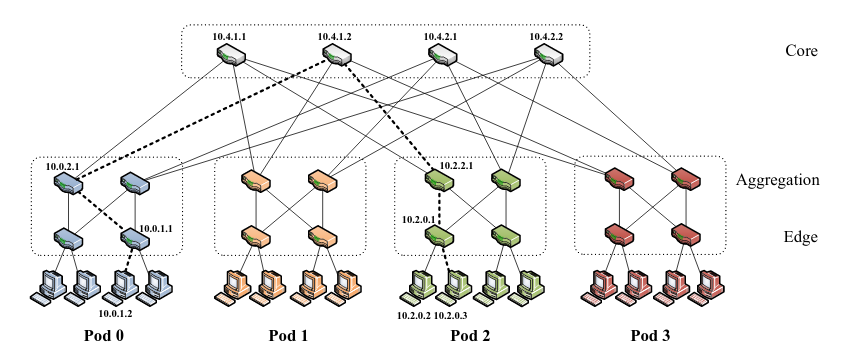
\includegraphics[width=\textwidth]{fat-tree}
    \label{fig:fat-tree}
    \caption{An example of a fat-tree topology from \cite{al-fares_scalable_2008}}
\end{figure}

The typical bandwidth vary but are in the 10Gbps to 100Gbps scale for these links.
Some networks assume different link speeds between the ToRs than from server to ToR, others are uniform.

The latencies involved are often extremely small, on the order of tens of nanoseconds.


\subsection{Traffic modelling} \label{model-traffic}

There are a few well studied datacenter traffic models (datamining, websearch, Chen Stefan Manya paper, more), with a common takeaway being that datacenter traffic is hard to predict.

Traffic distribution can be broken down into multiple dimensions: overall load, skeweness, and flow size distribution.


Overall load corresponds to how much traffic is being offered onto the network relative to how much capacity the network has.
It is important to note that this does not mean that the network is able to 100\% load, most networks are overwhelmed far before.
The reason for this is simple: if on average, it takes 4 hops to get to the destination, traffic is essentially being sent 4 times, making any load above 25\% impossible to satisfy.

The traffic may be fairly uniform, each sender and receiver being involved in traffic all around the datacenter, or very concentrated, with a few "hot" racks being very active with each other, the rest of the datacenter quiet.
Describing these patterns can become quite complex, as there may be multiple "hot" regions mostly not interacting with each other.
Throughput this thesis, and in most of the literature, we tend to be concerned about uniform traffic, and heavily skewed traffic. % is this true??

Finally, the flow size distribution corresponds to how big each flow is expected to be \cite{alizadeh_data_2010}.
Some workloads, such as websearch, consists mostly of many small flows.
Others, such as datamining, are comparatively much bigger.
Machine working loads also typically create a large demand, for example in a ring, using all the networking resources available.

\section{Simulation Model} \label{model-sim}

The datacenter model used by Rustasim was chosen to emulate closely that of Opera, to allow for comparison and verification of the results.

The model used in Rustasim \ref{rustasim}, consists of two actor types: routers and servers, and three model-level event types: \code{packet}, \code{flow} and \code{timeout} events.
The servers are organized in racks, themselves interconnected through a user-chosen topology.

A \code{packet} event carries with it the corresponding packet and signals the arrival of that packet to the actor who then forwards it along appropriately.
If the packet carried by the event arrives at its destination, it is acked.
If the packet is an ack arriving back at the sender, the flow reacts appropriately.\\
\code{Flow} events are received directly by servers and indicate the start of a new flow at that server.
\code{Timeouts} are received by the senders themselves and may cause a packet to be retransmitted if it hasn't been acknowledged.

Following with Opera's design, the queue sizes are TODO, the link speeds are all 10Gbps.
The latencies in the Opera simulator are set to 0 from server to ToR, and 500ns from ToR to ToR.
Unfortunately, conservative scheduling algorithms are unable to make progress with 0 latency, so I've set all latencies to be 500ns.
This has a measurable impact on the completion time of very small flows, where latency is the main contributor, but otherwise does not impact the results.
This is discussed more in section \ref{replication}.


\subsection{TCP} \label{model-tcp}

In this model, a limited version of TCP is implemented with a fixed congestion window of size 30, similar to choices Opera makes.
Although it is possible to implement a more realistic version of TCP, this simple version is close to the Opera simulator that the results check out.

\chapter{Simulator design} \label{simulators}

\section{RotorSim} \label{rotorsim}

RotorSim \cite{brode-roger_nibriviarotorsim_2020} is a centralized simulator (see \ref{centralized-sim}) of a packet-level datacenter network model (see \ref{model}).
It is implemented in Python \cite{van_rossum_python_2009} and is single-threaded. %does python need to be cited?

\subsection{Event queue} \label{rotorsim-eventq}
\subsubsection{API} \label{rotorsim-eventq-api}

\begin{table}[ht]
\begin{center}
\label{rotorsim-eventq-api:table}
\begin{tabular}{|p{1.8in}|p{3.8in}|}\hline
\code{create(limit)} & Instantiates an event queue with the given \code{limit} \\\hline
\code{call\_at(time, event)} & Schedules \code{event} at the specified \code{time} \\\hline
\code{call\_in(delay, event)} & Schedules \code{event} at the current time+\code{delay}  \\\hline
\code{run\_next()} & Starts the event simulator, returns when \code{limit} is reached, there are no events to run, or \code{stop()} is called \\\hline
\code{stop()} & Forces the event loop to return \\\hline
\code{time} & Returns the current time \\\hline
\end{tabular}
\caption{RotorSim event queue API}
\end{center}
\end{table}

The event queue allows for the addition of new events through two functions: \code{call\_at(time, event)} and \code{call\_in(delay, event)}.
These will then appropriately add the event to the queue and return.
The exact structure of \code{time} and \code{event} are discussed in \ref{rotorsim-eventq-event}.

To event loop is started through a call to \code{run\_next()} and finishes either when there are no more events to schedule, or when it hits a limit defined at its creation.
The loop may also ended by calling \code{stop()}, breaking the loop.
Although rarely useful when running simulations to produce results, it is useful while debugging.
After being stopped, the loop may be resumed through another call to \code{run\_next()}.

% wow is this section badly written
In order to make code more readable, and less error-prone, the module also exports a function decorator, \code{@delay(amount)} that will wrap a function in a call.
A useful case for this is to enforce delays in reconfiguration or receiving packets.
For example, if an switch $S$ has a \code{recv(packet)} function that processes incoming packets, it may be useful to wrap this with a \code{@delay(latency)}, enforcing that anyone calling the function waits an additional $latency$ amount.
Calling \code{S.recv(packet)} then doesn't actually call the function itself, but schedules an event $latency$ later that will call said function.
In practice, most calls are made this way, clearing the code of many \code{call\_in} statements.


% write up full example?


\subsubsection{Event structure} \label{rotorsim-eventq-event}
RotorSim's event queue is implemented using Python's \code{heapq} \cite{noauthor_heapq_nodate}.

Python tuples are ordered by comparing the first element of the tuple, going to the next in case of a tie.
This naturally leads to events being a tuple of time and event description.

Python allows for the treatment of functions as values, as well as for calling a function with an array, or a dictionary as arguments through the \code{*args} and \code{**kwargs} idioms.
Once the

In addition to \code{(time, function, args, kwargs)}, the event queue adds a user-controlled priority value to allow for the breaking of ties for events that happen simultaneously.
Although this isn't strictly required, it does simplify simulator design around configuration changes.
For example, if the routing table of a device changes and a packet sent, both at time 100, it is often intended that the configuration change take place before the packet is routed, avoiding odd situations where a packet is routed along a path that no longer exists.

Finally, as suggested in \code{heapq}'s documentation, there is a final integer, a counter, inserted after the priority. Ostensibly this breaks ties between events having the same time and priority by the order in which they are inserted.
This property is not used in the simulator, however it stops python from 

Each event is a tuple consisting of, in order, the current time, a priority (lower means run earlier), a unique counter, 



\subsection{Limitations} \label{rotorsim-limits}

There were two main frustrations with RotorSim, its large memory usage and "slow" performance.

\paragraph{Memory usage} \label{rotorsim-mem}
Large simulations used up a lot of memory.
Part of this is due to the large amounts of objects being actively used, see \ref{limits-mem}, but Python also offers little to no control of the underlying memory representations of objects.

\paragraph{Low performance} \label{rotorsim-perf}
In addition to large memory usage, it often took over 24h, sometimes even up to 72, to get results.
This significantly slows down the research iterations.
Although this was sometimes mitigated thanks to being able to run hundreds of simulations simultaneously, this was only interesting when we wanted to explore a large cross-section of different parameters.


\subsection{Python runtime} \label{rotorsim-runtime}

Different interpreters exist for the python programming language, the default being CPython.
However, I found that using PyPy \cite{team_pypy_2019} yields an almost 2x performance improvement for the simulator compared to CPython.
Even Pypy can run virtually all Python code, numpy \cite{van_der_walt_numpy_2011} is difficult to set up properly.
For RotorSim, numpy was only used for some random number generation, making moving away from the package easy.








\section{Rustasim} \label{rustasim}

Rustasim \cite{brode-roger_nibriviarustasim_2020} is a parallel discrete event simulator implemented in Rust \cite{klabnik_rust_2018}\cite{matsakis_rust_2014}, and heavily benefiting from the well-optimized data structures of the crossbeam library \cite{noauthor_crossbeam-rscrossbeam_2020}.

The main impetus for exploring a different programming language came from repeatedly hitting memory limits with RotorSim (even with 96GB of RAM!) and being frustrated at its slow speed.
A goal was proposed to make a simulator run medium-sized simulations within a few hours, yielding an objective of managing to simulate 100Gb worth of traffic moving for every wall-clock second the simulator is run.
For context, Rotorsim is able to move 126Gbps on a laptop, more in \ref{}.


\subsection{Language choice} \label{rustasim-language}

In order to achieve the desired goal, I decided to re-evaluate the choice of programming language.
Rotorsim used Python because it was chosen for a class project, which later turned into a research simulator.
There was no formal evaluation of that choice.

The evaluation criteria were a combination of resulting speed and ease of development.
The candidate languages were: Python, Go \cite{donovan_go_2015}, C \cite{kernighan_c_1988}, and Rust.
All but Rust were chosen due to my familiarity with them, Rust chosen because recommended to me.
Go was interesting due to potential for easy concurrency and parallelism.
C was chosen for its reputation as a high-performance language.

For each of the languages I implemented a simple simulator consisting of one device with a `loopback' link, a connection feeding right back to itself after a small latency.
The goal was simply to see how fast the simulator was able to be pushed, and how easy or not developping in the language was.
\begin{itemize}
\item Python took a few hours to re-implement, and was able to move 25Gb of traffic for every second of realtime on the link.

\item Go took almost a day, due to not having a generic function structure such as python, eventually solved through the use of closures.
However the performance was, surprisingly, nearly identical to python's at around 25Gbps on the same machine.
Attempts to make the simulation parallel, by processing the event and heap operations in parallel slowed down the simulator due to the need for synchronization between the different routines.

\item Rust took much longer to develop, around 4-5 days, most of which was spent getting familiar with a new memory management model.
Rust also does not take well to functions whose type is not defined at compile time, making calling arbitrary functions difficult.
However, Rust has structured enumerations, allowing all the different event types to be defined at compile time.
The event loop could then, on a pre-defined event, call a specific function.
Since the different enumeration variants can also carry distinct data, the arguments for the function can be carried with the variant, allowing flexibility in the types of functions called.
After some quick optimizations, Rust moved 125Gb per second, faster than goal.

\item The C implementation never took off, the library management system being difficult to manage, simple data structures like the heap requiring re-implementation.
\end{itemize}

Thus Rust became the top choice, despite a long implementation time, since I believed this was due to the initial learning cost, and not to a fundamental feature of the language.
In addition to switching to Rust, significant effort was put into parallelizing the simulation.
After having spent significant time developing the full simulator, that bet has proven correct, the language is very rarely what is holding development back.



\subsection{System overview} \label{rustasim-overview}

\begin{figure}[h]
\centering
\label{rustasim-overview:fig}
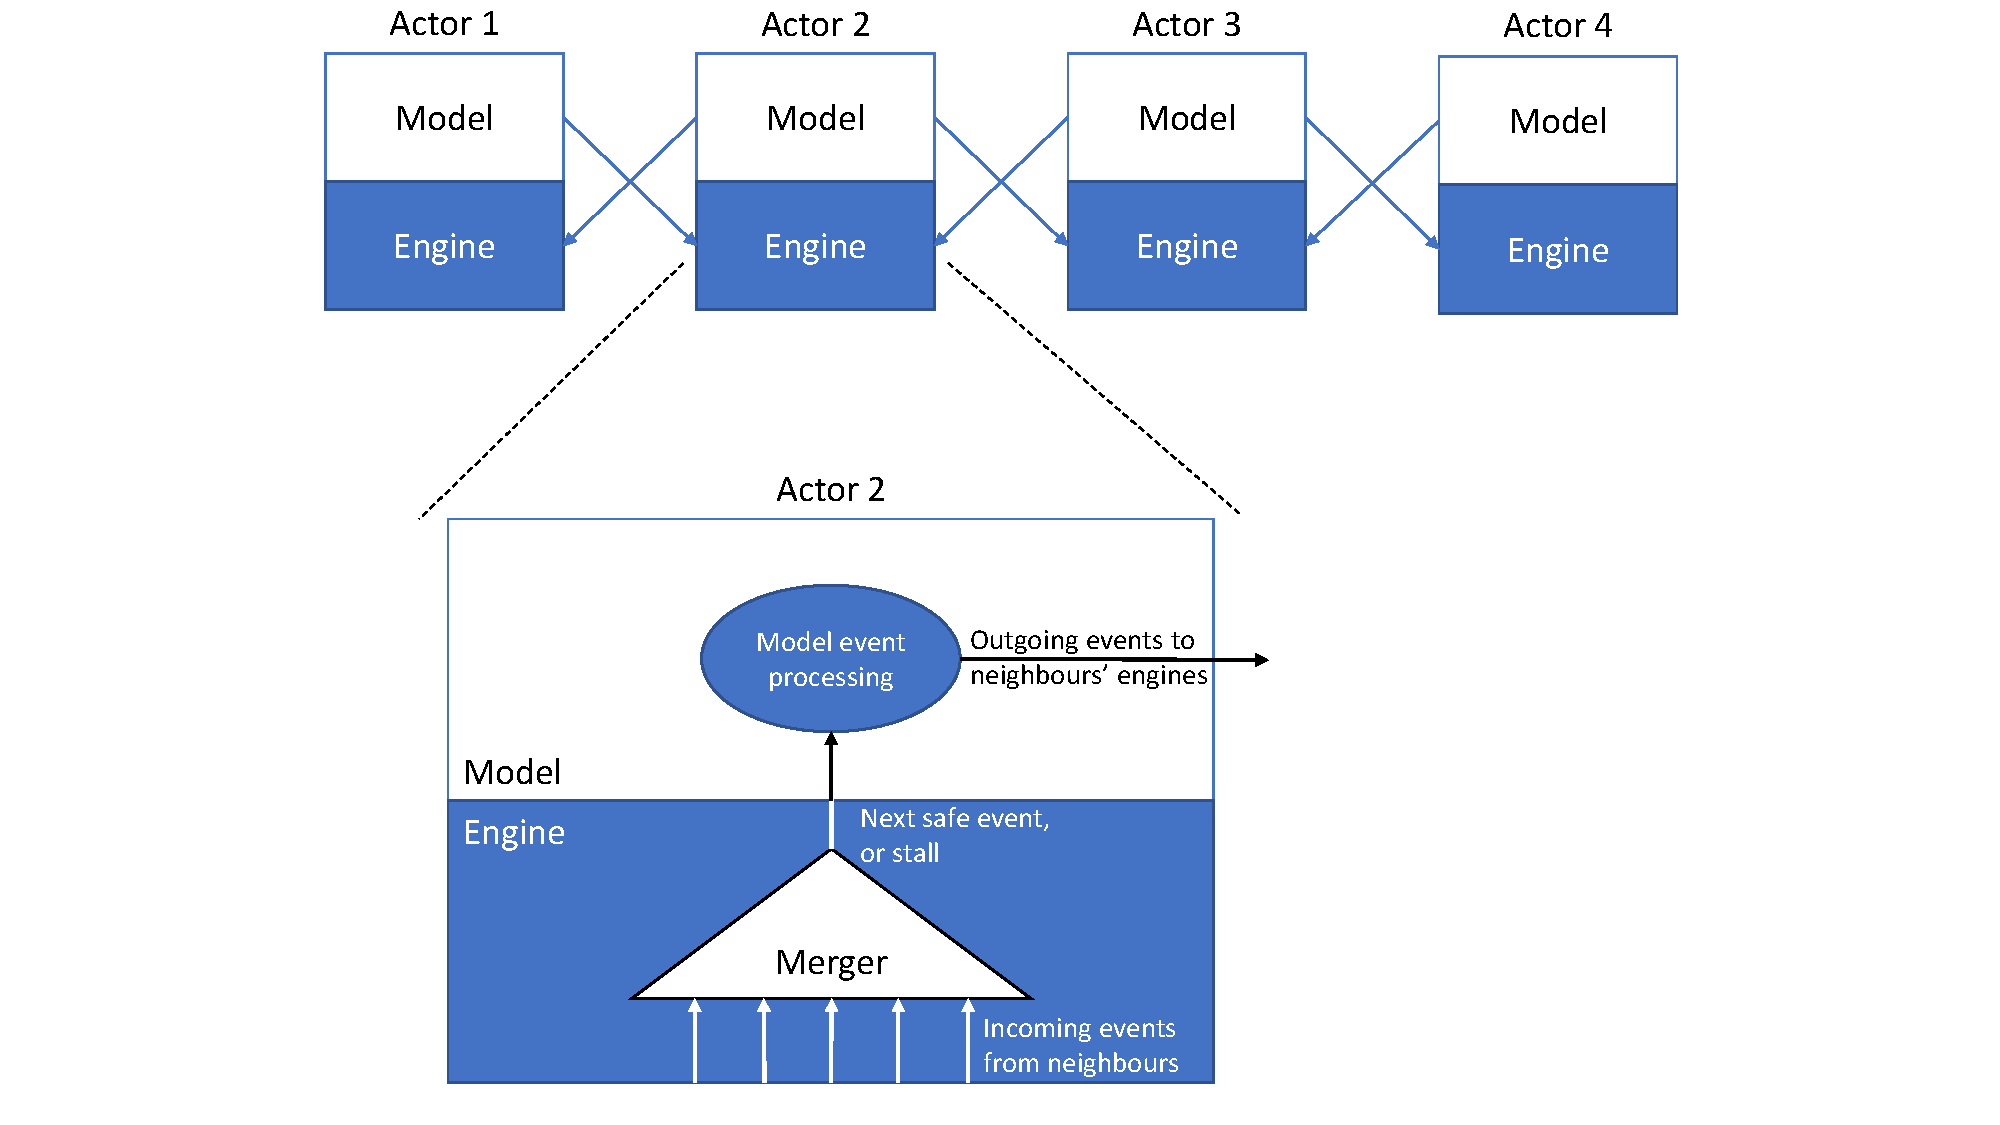
\includegraphics[width=\textwidth]{system-diagrams}
\caption{Rustasim actor overview}
\end{figure}

A Rustasim simulation consists of many actors, each running concurrently, not necessarily simultaneously, to all others.
This concurrency brings with it all the challenges described in section\ \ref{pdes}: preserving causality and guaranteeing progress.

To make developing models easier, Rustasim enforces a separation between the model and the code that deals with the parallel aspects of the simulation, the `engine'.
The engine and the model then have a application/system relationship: the engine receives all incoming events, arranges them in order and detects stall, returning to the user/model the events in order.
This is abstraction very similar to how applications interface with TCP: the application receives the bytes in-order while the OS handles the complexities of re-ordering and managing the connection.
The actor receives the events in order through an iterator, matches on the event type and executes the appropriate action.
It is required to take certain actions upon receiving certain events

Since there may be thousands or more of actors, it is not possible to spin up separate threads for each of them.
Instead Rustasim spins up as many worker threads as there are available cores, and actors are scheduled on the workers.
The details of the scheduling are described in \ref{rustasim-sched}.



\subsubsection{The actor-engine abstraction} \label{rustasim-actor-engine}

The events in a distributed simulation are slightly more complex than in a centralized one.
Although most events processed by actors, are still model events, there is a need for additional event types in order to guarantee progress.\\
\code{Null} events are required to signal neighbours that it is safe for them to progress up to a certain time without waiting for this actor.
Without these messages, an actor cannot be sure if the silence from the neighbour comes from a lack of events to send, or from a delay in computation.
Although \code{Null} events are required to guarantee progress, actors will never receive them: they are only useful for the engine to progress, the actor need not take action on them.
The sole purpose of \code{Null} events is to allow the neighbours' engines to make progress.\\
Because the \code{Null} events require model-level knowledge to send, the engine cannot do so on its own.
However, it is the engine that will become aware of a potential deadlock, not the actor.
Therefore, to inform the actor of a potential stall, the engine generates a \code{Stalled} event.
Upon receiving such an event, the actor is \emph{required} to send all necessary neighbours a \code{Null} event updating how far they may progress.
If a neighbour has already received another event at, or past, the time the \code{Null} event would be received, the \code{Null} event is not sent.\\ %TODO make clearer
Finally, \code{Close} events tell the actor to return from its event loop.
Although this might seem trivial, it does require a little care, it is easy to leave the simulation hanging at this point.
It is necessary to also inform neighbours that we have no more events to communicate to them.
This can be done by sending \code{Null} events that pass closing times, or by sending \code{Close} events to the neighbours.

% TODO re-write, more details, reorgnize, cite?
\paragraph{Compiler enforcement}
By separating the actor and the engine into different crates, the modularity is strictly enforced by the Rust compiler, forbidding the simulator designer from modifying the internals of Rustasim.
In order to allow for arbitrary models to be built on top of Rustasim, the events the engine deals with are parametrized through a generic type \code{T}.
Because the engine code is generic over \code{T}, it cannot make any assumptions about what the type looks like, lest the Rust compiler errors.
However, when compiled, the compiler will fill in the type appropriately and is able to optimize as though the type were written explicitly written in.\\
This separation between the model and the engine also allows for many different models to be implemented using the same engine, allowing for significant reuse between projects.
This is particularly appealing because most optimizations are implemented in the engine itself, and allowing further optimizations to be propagated to many simulations.
This separation also allows the writing of tests for the engine using a trivial model, making it easier to validate the engine and catch subtle errors.

\subsection{Message passing} \label{rustasim-message-passing}

The communication between actors is done through a single-producer, single-consumer channel.
Rust offers a default channel implementation for multiple-producers and a single-consumer, which although technically correct isn't performant enough.
Multiple Rust crates offer more performant options, and after testing many different options, including Ringbuffer (TODO cite), crossbeam's (TODO cite) channels, the most performant option was the unreleased single-producer single-consumer queue from crossbeam.
In order to be easily published, Rustasim currently extracts the SPSC channel code from the unreleased branch of crossbeam.

\subsection{Multi-queue merging} \label{rustasim-tree}

This is the core of the engine: merging multiple queues together, and returning the next event if it has heard from all neighbours, as described in \ref{null-messages}.
If a neighbour has not been heard from, the scheduler should return a \code{Stalled} event.

\subsubsection{An initial approach: heaps}
An initial approach might be to maintain a heap of all received event along with a counter for the number of events in the heap from each sender.
The running time for this structure is sub-optimal, since it grows with to the amount of events in the queue, which is, due to the nature of waiting on everyone, always going to be nearly equal to, or greater than the number of neighbours.
The algorithmic complexity of processing or returning an event is then $O(\log e)$, with $e$ being the number of events in the queue.

An improved approach would take only the top event from each of the senders and maintain a heap of those.
The heap is then bounded by the number of senders, and the book-keeping is reduced to whether or not a sender has an element in the heap.
This structure then has an algorithmic complexity of $O\left(\log n\right)$
This works relatively well and does slightly improve running time.

When waiting on a neighbour, i.e. there are no events from at least one actor in the heap or in the incoming queue, the merger returns a \code{Stalled} event.
Otherwise, the merger returns the smallest current event off the heap, and attempts to extract an event from the incoming queue.
If there are no events in that neighbour's queue, the neighbour is marked as missing and the merger may stall when asked about the next event.

It is not necessarily true that marking a neighbour as missing results in a stall: it is possible that by the time the next event is requested from the merger, another event has been sent.
It is also possible that there is another event, from a different neighbour, that has the same time.
These tied events are all safe to return, and returning tied events can limit the number of stalls and increase performance.
This means that there may be more than one neighbour marked as missing without there being a stall.

\subsubsection{Loser trees}

Although there does not exist to my knowledge a structure with a better algorithmic performance, there exists structures with significantly better constant factors.
Notably, general purpose heaps can grow and shrink in size, and are non-monotonic: they do not require the input to be continuously growing to properly work.
By taking advantage of these two restrictions, we can reduce the complexity of the heap and dramatically increase the performance of the merger.
In some experiments, improvements can be greater than a factor of 2 over the heap.

Notably, this problem is essentially identical to the problem of merging tapes: there is a fixed number of tapes, and the reader cannot look ahead in the data, and we are required to assume the data on a single tape is already sorted.
Tournament trees in particular solve this problem elegantly.

A tournament tree takes in a certain number of elements to compare, here the next element of each of the queues and pairs them off.
The winner of each exchange, the event to be scheduled the soonest, moves on to fight another winner.
This process eventually forms a tree analogous to the structure of many tournaments.
Although it may be natural to record the winner of each exchange, recording the looser makes for a significantly more elegant algorithm as described by Knuth \cite{knuth_art_1998}.

\begin{figure}[h]
    \centering
    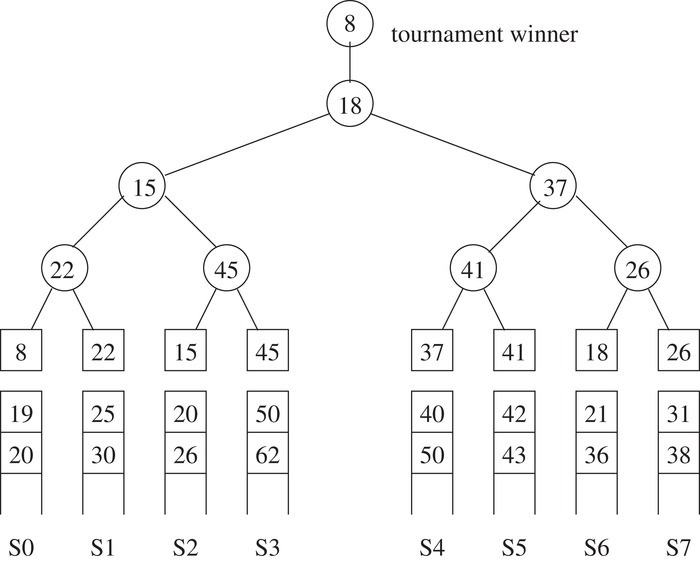
\includegraphics[width=\textwidth]{loser_tree}
    \caption{Loser tree example from TODO}
    \label{loser-tree:fig}
\end{figure}

In the example of Figure \ref{loser-tree:fig}, the current winner is 8, coming from \code{S0}.
In order to find the next smallest value, which a quick visual scan reveals should be 15 from \code{S2}, we re-run all the tournaments starting from \code{S0}.
The new value of \code{S0} is now 19, which goes up against the currently saved value in the parent: 22.
18 wins and moves on to go up against 15, which it loses.
Upon losing, we swap the two players, writing 18 down in the place of 15, and continuing 15 up the tree.
Reaching the root node of 18, current player 15 wins and is now the tournament winner.


\paragraph{Dealing with ties}
In order to allow tied events to be returned before a stall, when an incoming queue doesn't have any events to insert into the tree a \code{Stalled} event is inserted in its place.
The inserted event will then make its way to the top of the tree as though it were any other event, being returned when it is its time.
However, this alone doesn't mean all tied events will be returned, in order to guarantee that, \code{Stalled} events lose to events that are at the same time.

It is also important not to spuriously return a \code{Stalled} events: doing so will cause the actor to do expensive actions, and will upset the scheduling process described in \ref{rustasim-sched}.
When a \code{Stalled} event wins, the merger checks the neighbour's queue again and if it is no longer empty, will not return the \code{Stalled} event and will continue the process with the new event.


\subsection{Scheduling} \label{rustasim-sched}

\begin{figure}[h]
    \includegraphics[width=\textwidth,page=2]{system-diagrams}
    \caption{Rustasim actor overview}
    \label{rustasim-scheduling:fig}
\end{figure}

In the cases where there are less actors than available cores and there isn't contention on the system (no other CPU heavy job), it is possible to give each actor its own thread and still have excellent performance.
In this scenario when an actor stalls and is waiting on another, it can `busy-wait', burning CPU cycles until there is a new event on the channel.
More subtle synchronization primitives could be used, but all have some overhead, whereas checking in a tight loop has none.

However, The huge disadvantage of busy-waiting is that it gives the operating system no help as to which thread should be scheduled next, often scheduling threads that have nothing to do but burn cycles.
This issue alone is enough to make the simulator over 1,000x slower.
Explicitly yielding the thread on a stall sometimes improves the situation, but not much, since the OS still has no clear idea of who is best to schedule next.
In fact, cursory experiments suggest that it often repeatedly picks the same threads to schedule, letting it advance ahead of the rest, stall, and get rescheduled soon after, making little progress before stalling again, and so on.
Unfortunately switching between threads is an expensive operation for the operating system, and can easily take up a huge fraction of the simulation time.
In some runs, thread-switching took up almost two thirds of the simulation time, i.e. removing the scheduling issue could speed up the simulation by a factor of 3.
In addition to the overhead of thread switching, repeatedly stalling an operation sends out more \code{Null} events than necessary: they were not sent because of a deadlock, but because of a scheduling issue, creating overhead.
On its own, sending more events than needed may not seem like a big issue, they are cheap to process, but these \code{Null} events can become the main event type the stragglers receive, sometimes exceeding half of all received events.
\\


However, a better setup would be to have as many active actors as available cores, and to always schedule the most-straggling actor.
Indeed, being last means that the actor can run for longer uninterrupted, reducing the overhead of scheduling actors.

An easy way to schedule actors is such a pattern is to advance an actor until it stalls, then schedule every other actor, guaranteeing that the current actor is `last' before scheduling it again.

This can be done by having a single shared queue shared behind a lock, workers popping the front of the queue and pushing stalled actors at the back.
However, this queue then becomes a contention point between the actors.
This can be mitigated by having a few queues each with its own lock, and having workers randomly picking a queue and popping an event from it after pushing the stalled actor onto it.

\begin{figure}[h]
    \centering
    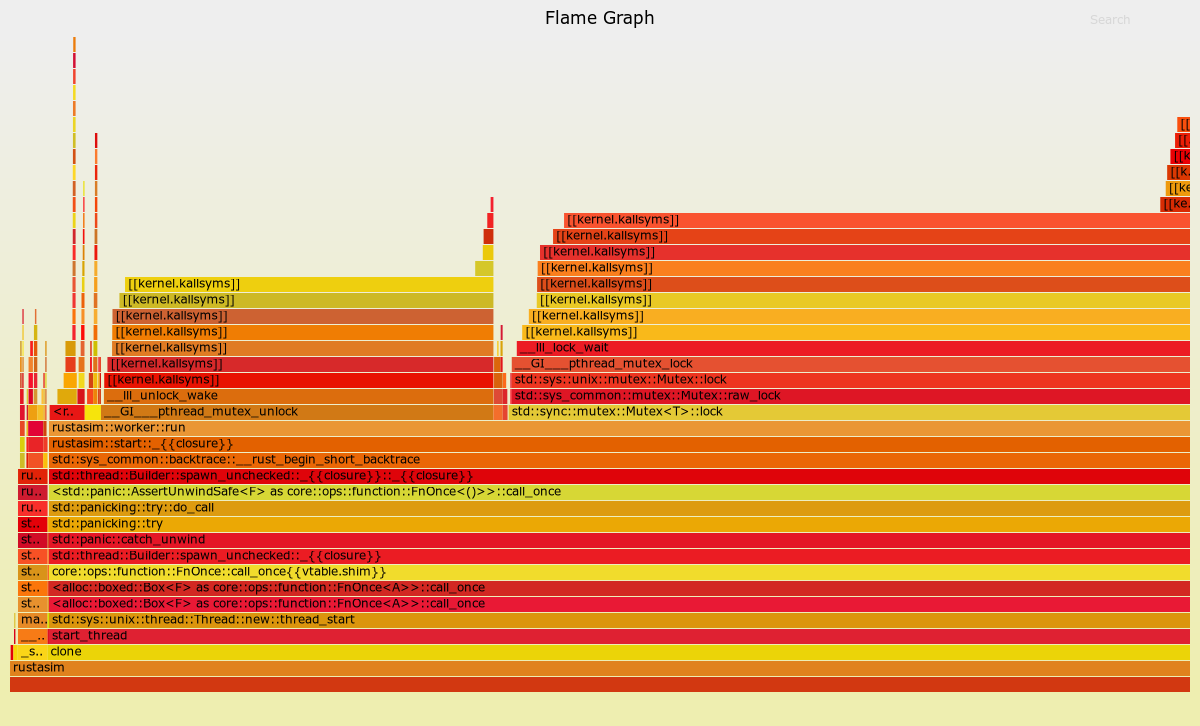
\includegraphics[width=\textwidth]{flame-lock-one-heap}
    \caption{`Flamegraph' of a Rustasim run with a single shared scheduling queue: lock contention accounts for over 90\% of the runtime.} %TODO cite
    \label{rustasim-lock-one-heap:fig}
\end{figure}

It is possible to push and pop from two distinct random queues, but this has the disadvantage of acquiring two locks for every scheduled actor and of allowing queues to drift to different sizes.
Pushing and popping from the same queue does not change the size of the picked queue since it both adds and removes an element from the queue before releasing it, and only acquires one lock.

Initializing and terminating the scheduler requires a little care: since the number of elements in the queues won't change size during the course of the program, they should all start with roughly the same number of actors each.
Failure to evenly distribute the queues may result in some actors being rescheduled too quickly or too slowly depending on if they end up in a shorter or longer queue, hurting performance.

Terminating the process is tricky: a single queue being empty indicates that some actors have finished, but does not indicate that all have.
In order to know when to terminate, a shared global counter is created which is incremented every time an actor finished.
When the shared counter reaches the number of actors, all actors are done and the workers can safely finish.
\\

In order to support this kind of scheduling, when actors are scheduled, they are required to only make progress as far as they can.
Once a \code{Stalled} event is received, they must return to let other actors be scheduled.
To allow the workers to distinguish a finished actor from a stalled actor, the actor returns either an \code{ActorState} which is either a \code{Continue(T)} containing the furthest time the actor got to, or a \code{Done(R)} containing the final result of the actor.
Although unused in this scheme, the furthest time reached by an actor can be used by more complex schedulers to further optimize the simulator's scheduling.

\subsection{Timeouts} \label{sim-timeouts}

Timeouts are by the nature of their generation, a little complicated to schedule in the simulator.
In order for an actor to send an event to itself, it must have itself as a neighbour.
In practice, this means that there is a queue whose receiving engine is the actor's own engine.

However, because timeouts can be generated for different values at different times, it is entirely possible for a timeout generated after a previous one to finish before the earlier one.
This out-of-order property means that we cannot simply use the event-merger to re-order the timeouts properly.
However, this can be solved by making use of the fact that timeouts have a large minimum value, a good fraction of a millisecond.

Instead of being sent to the actor, timeouts generated by a server are kept in a local heap, and a "check for timeout" event is sent to the engine.
Upon receiving the timeout, the server checks to see if any timeouts need to happen, and executes those.
The server also then schedules the next "check for timeout" event at that point.

Scheduling the "check for timeout" event is done by checking when the next timeout is scheduled to happen.
If the next timeout is going to happen sooner than any other timeout, i.e. it is scheduled to happen less than the mimimum timeout away, the checking event is scheduled for when the next timeout expires.
If the next timeout will expire longer than the minimum possible timeout in the future, the server schedules a check for a minimum timeout in the future: this will catch all fast timeouts which may generated before the current next timeout will expire.

Although this might seem slightly convoluted, this design for timeouts is efficient and highlights the flexibility of Rustasim in implementing patterns that may not seem to be part of its paradigm.


\subsection{Indexing} \label{rustasim-indexing}
% Not sure where this section best goes...

Although most programs consider the performance cost of a hash to be negligible, at the scale of nanoseconds, it becomes noticeable.
There is therefore a large incentive to not use hash tables and rely on the significantly faster direct indexing offered by arrays.
However, most data structures maintained by both the actor require indexing by the neighbour's \code{id}.
This \code{id} is unique across all actors and is useful for routing and for keeping track of who an event's sender is.

An alternative to structuring these data by \code{id} is to add every neighbour to an array and refer to them by their index.
Unfortunately that mapping isn't going to be regular across all actors, and some structure still explicitly require an \code{id}, notably packet destinations.

In order to minimize the amount of hashes to be made, each actor keeps track of a single hash table that maintains a translation from \code{ids} to an index \code{ix}, as well as an array containing an \code{ix} to \code{id} translation, mostly used for debugging purposes.
In addition, if the \code{id}s of all the devices in the network are continuous starting from 0, the routing table can be indexed, not hashed, by \code{id}, and return the appropriate index.

However, it is possible to avoid hash table lookups entirely with the cooperation of the engine.
The engine doesn't care about the model \code{id} of its neighbours, it only needs to receive its events.
By having the engine maintain the incoming queues in an array the same order as the actor has setup its \code{id}s, it is possible to translate the source \code{id} of the event to an index without needing a lookup.
Indeed, when the engine removes an event from a queue, it necessarily knows the index of that queue in its array of incoming queues.
It can then overwrite the incoming event's source field with the appropriate index, no lookup required.

Flows follow a similar pattern and are given a \code{flow\_id} only by the source server, akin to how TCP ports are used in the real world.
Each \code{flow\_id} can then simply be an index into an array, limiting the need for hash tables entirely.

The combination of these optimizations mean that there is almost no need to execute a hash table lookup in the normal processing of events.
The full translation tables, although never used in a proper simulation run, can be extremely helpful in debugging.


\chapter{Simulator limits} \label{limits}

In this chapter we explore theoretical limits of simulators both in terms of speed, and what is even feasible.
\\

Throughout this chapter, the baseline model will consist of 4,773 actors comprised 128 racks connected to 37 backbone switches and 37 servers each through bidirectional 10Gbps links.
The full bandwidth of the network is therefore $2\times128\times(37+37)\times10Gbps = 190Tbps$, over 10 simulated seconds this corresponds to up to almost 2,000Tb of data.
The packet size will be assumed to be 1,500~bytes, the TCP standard. \\
Note that network speeds are typically measured in bits per second, not bytes.
For more details on the structure of datacenters see section \ref{model-dc}.

\section{Memory feasability} \label{limits-mem}

The main limiting factor in the feasability of simulations is memory consumption.
Speed is typically not a concern since it is always possible, if frustrating, to wait longer.
Storing the results of a large simulation could also be limiting but disk space is relatively cheap.

There are three main sources of memory usage in this simulation: events, packets, and flows.
Although there are nearly 5,000 actors, they each (without their events, packets, and flows) take up fairly little memory.
Even if they each took up a full 10 kilobytes, this would correspond to 50MB of RAM, barely noticeable on today's computers.

\paragraph{Packets}
A fully saturated network on the model above will result in 16 billion packets being sent for every simulation second.
Each packet contains information about its source, destination, size, the flow it belongs to, and so on...
%mark

\paragraph{Events}

\paragraph{Flows}


\section{Speed} \label{limits-speed}

\paragraph{Metrics}
In order to more easily compare the speed of different simulators, it is useful to talk about the amount of simulated data moved per real second.
Since this metric has units of data over time, I will refer to it as the simulator's bandwidth.
As a useful reference, a simulation bandwidth of 100Gbps results in a running time of 5.5h for a typical 10s run.

A more standard metrics is the number of events per second that the simulator executes.
It is less useful here since it doesn't directly translate to how long the simulator runs, it can also be highly dependent on the type of events being processed.


\subsection{Processing power} \label{limits-cpu}

In the worst case scenario, the network is fully saturated, meaning that the 190Tbps of the network are filled with packets.
This corresponds to 16 billion packets per simulated second (16Gp/s), meaning at least that many events.

If a packet takes around 100 CPU cycles to process on average, which is an optimistic guess: a single L2 cache access takes around 10 cycles, on a 2GHz CPU that corresponds to 50ns of processing per packet, or 20 million simulated packets per real CPU-second. % TODO cite cache speed
Although this may seem slow compared to the 16Gp/s of the network under simulation, this corresponds to a simulation bandwidth of 240Gbps.

Optimistically, across multiple CPUs, we can hope to multiply this effect.
My laptop's 8 cores may therefore dream of running a simulation at nearly 2Tbps.

Realistically, 100 cycles per packet is optimistic, and in the case of a parallel simulaiton, the synchronization between cores becomes expensive: a typical shared lock operation alone typically taking 20-30ns. %TODO cite
These numbers do allow us to understand an upper bound of what is possible.



\subsection{I/O} \label{limits-io}

The slowest component of a computer is always the IO interface, and the entire point of running simulations is to have a record of what happened during the running of it.
It is therefore necessary to log particular events during the running of the simulation.

Since I am interested in finding upper bounds, I will be particularly generous in the encoding schemes proposed.
In practice, I expect these data to take up more space than I propose, but these calculations serve to limit our dreams and not necessarily indicate what is realistic.

\paragraph{Packet-level logging}
The highest level of detail can be measured by logging every single packet movement.
The bare minimum needed would be to log some form of packet identifier and a source and destination.
Given 5,000~hosts, the source and destination can each have 16~bits of a 32~bit integer.
However, uniquely identifying the packet is tricky, but a 64~bit integer should theoretically be enough.
This results in 12~bytes of data per packet movement, and a logging bandwidth of almost 200GB per simulated second.

The fastest SSDs advertise writing rates around 500MBps, which if fully utilized yields a maximum simulation rate around 500Gbps.
However, the amount of data generated under this scheme is large: it is typical to run dozens of simulations for a single plot, and under this logging scheme and nearly magical encoding, each run would produce nearly 2TB of data.

However, this calculation illustrates that IO is not as much of a limit as might be expected: 500Gbps is twice as high as the single-CPU limit of section \ref{limits-cpu}.
Fortunately for us, IO is even less of an issue if we log less data.

\paragraph{Flow-level logging}
We can significantly reduce our IO needs if instead of logging each packet, we log only the flows, along with its source, destination, size, and duration.
The source and destination can again both share a 32~bit integer.
However, the size of the flow in simulation can vary from a few KB to GBs, a range that can barely fit in 32~bit values.
Time in the simulator is measured down to the nanosecond, but such precision is not required, allowing it to also fit in a 32~bit value.
This brings the overall size of logging a single flow to three 32~bit values, or 12~bytes.

The last value that is required to compute this limit is the average flow size.
However, this is highly dependent on the traffic distribution (see \ref{model-traffic}).
The datamining workload has an average flow size around 62Mb, a small distribution we use internally has an average of 1.5Mb, while another one has an average of 1,100Mb.

With the smallest average flow size of 1Mb, we will be producing over 2GB per simulated second of log data, which, consumed at 500MBps supports simulation speeds up to 40Tbps.
Datamining can be simulated up to 2,500Tbps, and the largest distribution up to 45Pbps.
In other words, IO is not the limiting factor.



\chapter{Experiments and results} \label{results}

\section{PHOLD performance} \label{phold}

A standard measure for the performance of parallel distributed simulators is the PHOLD benchmark %TODO cite
It is a parallel version of the HOLD benchmark. %TODO cite

The HOLD benchmark consists of a certaim amount of original events, which, when processed, would schedule another one some random amount of time in the simulation future.
Typically the distribution of time before a next event is processed is an exponential distribution although that may vary.

A PHOLD benchmark follows the same idea, with the only difference being of which actor receives the event.
Instead the actor may be the same as the processing actor, or a different one (or `remote' in PHOLD terminology).
The fraction of remote events is an input parameter for the PHOLD model.

In addition to the number of remote events, there is also a parameter controlling the minimal amount of time before another event is scheduled.
This value, called the \code{lookahead} represents a form of latency between actors and is necessary for conservative simulations to make progress.


\begin{table}
\begin{center}
\label{phold-params:table}
\begin{tabular}{|p{1.8in}|p{3.8in}|}
    \hline
    \code{n\_actor} & Number of actors \\\hline
    \code{n\_events} & Number of initial events per actor \\\hline
    \code{n\_cpus} & Number of processing elements \\\hline
    \code{remote} & Fraction of remote events \\\hline
    \code{lookahead} & Minimum time before the next event is scheduled\\\hline
\end{tabular}
\caption{PHOLD parameters}
\end{center}
\end{table}
%XXX

\section{Network simulation performance} \label{phold}

Although general performance metrics are useful to compare against other general purpose simulators, Rustasim outperforms datacenter network simulators directly.
The other 

\chapter{Conclusion} \label{conclusion}
%\appendix
%\chapter{Tables}

\begin{table}
\caption{Armadillos}
\label{arm:table}
\begin{center}
\begin{tabular}{||l|l||}\hline
Armadillos & are \\\hline
our	   & friends \\\hline
\end{tabular}
\end{center}
\end{table}

\clearpage
\newpage

%\chapter{Figures}

\vspace*{-3in}

\begin{figure}
\vspace{2.4in}
\caption{Armadillo slaying lawyer.}
\label{arm:fig1}
\end{figure}
\clearpage
\newpage

\begin{figure}
\vspace{2.4in}
\caption{Armadillo eradicating national debt.}
\label{arm:fig2}
\end{figure}
\clearpage
\newpage

%% This defines the bibliography file (main.bib) and the bibliography style.
%% If you want to create a bibliography file by hand, change the contents of
%% this file to a `thebibliography' environment.  For more information 
%% see section 4.3 of the LaTeX manual.
\begin{singlespace}
\bibliography{main}
\bibliographystyle{plain}
\end{singlespace}

\end{document}

